%\part{Einfuehrung} 

%----------------------------------------------------------------------------
\section{Vorraussetzungen}

\begin{frame}
	\frametitle{Vorkenntnisse aus dem vorherigen Semester}
	\begin{itemize}
	  \begin{item}
	  	Sprechen Sie Java?
		  \begin{itemize}
			  \item Was sind Datentypen und Variablen?\linebreak
			  \item Kennen Sie Ausdr\"ucke?\linebreak
			  \item Wie werden Operatoren genutzt? Welche gibt es?\linebreak
			  \item Wann und wie werden Kontrollstrukturen eingesetzt?\linebreak
			  \item Was sind Bl\"ocke?\linebreak
	  	  \end{itemize} 
	  \end{item}
	\end{itemize}
\end{frame}
 
\begin{frame}
\frametitle{Ihre Erwartungen an die Veranstaltung}
	\begin{exampleblock}{Was m\"ochten Sie gerne behandeln?}
		\begin{itemize} 
			 \item{}
			 \item{}
			 \item{}
			 \item{}
			 \item{}
		\end{itemize}
	\end{exampleblock}
\end{frame}

\begin{frame}
\frametitle{Erwartungen an die Veranstaltung}
	\begin{block}{Was sollten Sie am Ende k\"onnen?}
		\begin{itemize}
			 \item{OOP verstehen und darstellen k\"onnen}
			 \item{Konzepte der OOP erl\"autern und anhand von Code darstellen}
			 \item{Die OOP bei der Softwareentwicklung richtig einsetzen}
			 \item{Weiterf\"uhrende Konzepte und L\"osungen der OOP verstehen}
			 \item{Die Grundlagen von Java als Werkzeug der OOP beherrschen}
		\end{itemize}
	\end{block}
\end{frame}

%----------------------------------------------------------------------------
\section{Werkzeuge}
\begin{frame}
\frametitle{In der Veranstaltung verwendete Werkzeuge}
	\setbeamerfont{block title}{size=\scriptsize}
	\begin{columns}[T]
	    \begin{column}{.3\textwidth}
	    	\begin{block}{Programmiersprache}
	    		\center
	    		
\includegraphics[width=1\textwidth, keepaspectratio=true]{bilder/java.jpeg}
	    	\end{block}
	    \end{column}
	    \begin{column}{.3\textwidth}
	     	\begin{block}{Entwicklungsumgebung}
	     		\center
	     		
\includegraphics[width=1\textwidth, keepaspectratio=true]{bilder/eclipse.jpg}
	    	\end{block}
	    \end{column}
	    \begin{column}{.3\textwidth}
	    	\begin{block}{Modellierung}
	    		\center
	    		
\includegraphics[width=1\textwidth, keepaspectratio=true]{bilder/uml.png}
	    	\end{block}
	    \end{column}
	\end{columns}
	\setbeamerfont{block title}{size=\normalsize}
\end{frame}
 
\subsection{Programmiersprache}
\begin{frame}
\frametitle{Warum Java?}
	\begin{block}{Java ist\ldots}
 		\begin{itemize}
		  \item Weit verbreitet.
		  \item Verh\"altnism\"a"sig leicht zu erlernen.
		  \item Plattformunabh\"angig.
		  \item Objektorientiert.
		\end{itemize} 
	\end{block}
	\begin{exampleblock}{Dokumentation}
		\url{http://docs.oracle.com/javase/7/docs/api/}
	\end{exampleblock}
\end{frame}
 
\subsection{Entwicklungsumgebung}
\begin{frame} 
\frametitle{Eclipse erleichtert uns die Entwicklung}
	\begin{columns}
	    \begin{column}{.5\textwidth}
			\small
			\begin{itemize}
			  \item Integrated Development Environment
			  \item Verwaltet Dateien in Projekten
			  \begin{item}
			  		Es existieren 4 Hauptkomponenten:
					\begin{enumerate}
					  \item \tiny Workspaces
					  \item \tiny Projekte (Projects)
					  \item \tiny Perspektiven (Perspectives)
					  \item \tiny Sichten (Views)
					\end{enumerate}
			  \end{item} 
			\end{itemize}
			\normalsize
	    \end{column}
	    \begin{column}{.5\textwidth}
	   		\center
	    	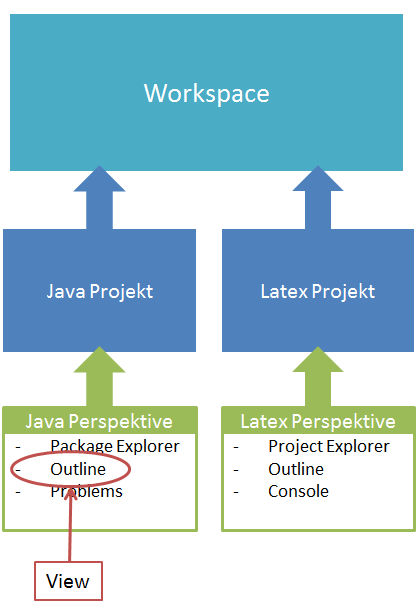
\includegraphics[width=1\textwidth, keepaspectratio=true]{bilder/workspace.png}
	    \end{column}
	\end{columns}
\end{frame}

\subsection{Modellierung}
\begin{frame}
\frametitle{UML unterst\"utzt bei der Darstellung der OOP}
	\begin{columns}
	    \begin{column}{.5\textwidth}
			\small
			\begin{itemize}
			  \item Unified Modeling Language
			  \item Sprache zur objektorientierten Modellierung
			  \item Standardisiert von der OMG
			  \item Auch zur Implementierung genutzt
			\end{itemize}
			\normalsize
	    \end{column}
	    \begin{column}{.5\textwidth}
	   		\center
	    	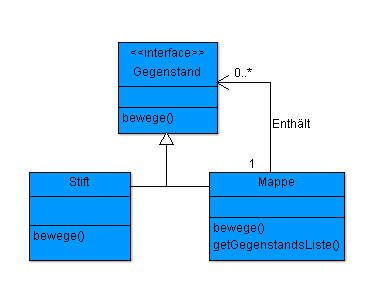
\includegraphics[width=1\textwidth,
	    	keepaspectratio=true]{bilder/uml_example.png}
	    \end{column}
	\end{columns} 
\end{frame} 
